\documentclass{article}

% if you need to pass options to natbib, use, e.g.:
% \PassOptionsToPackage{numbers, compress}{natbib}
% before loading nips_2017
%
% to avoid loading the natbib package, add option nonatbib:
% \usepackage[nonatbib]{nips_2017}

\usepackage{nips_2017}

% to compile a camera-ready version, add the [final] option, e.g.:
% \usepackage[final]{nips_2017}

\usepackage[utf8]{inputenc} % allow utf-8 input
\usepackage[T1]{fontenc}    % use 8-bit T1 fonts
\usepackage{hyperref}       % hyperlinks
\usepackage{url}            % simple URL typesetting
\usepackage{booktabs}       % professional-quality tables
\usepackage{amsfonts}       % blackboard math symbols
\usepackage{nicefrac}       % compact symbols for 1/2, etc.
\usepackage{microtype}      % microtypography
% set imports
\usepackage{ntheorem}       % theorem writing
\usepackage{cleveref}       % clever references
\usepackage{graphicx}       % for images
\usepackage{subcaption}        % images
\usepackage[table,xcdraw]{xcolor} % for tables
\usepackage{natbib}            % bibliography

% set paths
\graphicspath{{./figures/}}

\title{Interesting properties of GAN samples}
% The \author macro works with any number of authors. There are two
% commands used to separate the names and addresses of multiple
% authors: \And and \AND.
%
% Using \And between authors leaves it to LaTeX to determine where to
% break the lines. Using \AND forces a line break at that point. So,
% if LaTeX puts 3 of 4 authors names on the first line, and the last
% on the second line, try using \AND instead of \And before the third
% author name.

\author{
  Rafael Valle \\
  Center for New Music and Audio Technologies \\
  UC Berkeley \\
  Berkeley, 94709 \\
  \texttt{rafaelvalle@berkeley.edu} \\
  \And
  Wilson Cai\\
  UC Berkeley\\
  \texttt{wcai@berkeley.edu} \\
  \And
  Anish Doshi\\
  UC Berkeley\\
  \texttt{apdoshi@berkeley.edu} \\
  %% \And
  %% Coauthor \\
  %% Affiliation \\
  %% Address \\
  %% \texttt{email} \\
  %% \And
  %% Coauthor \\
  %% Affiliation \\
  %% Address \\
  %% \texttt{email} \\
}

\begin{document}
% \nipsfinalcopy is no longer used

\maketitle

\begin{abstract}
    In this paper we investigate numerical properties of samples produced 
    with adversarial methods, specially Generative Adversarial Networks. We
    analyzep pixel value statistics of real and fake data and compute distances based on the 
    marginal distribution of perceptually significant features. We provide results 
    on MNIST, music and speech data and show that GAN generated samples have 
    interesting signatures that can be used to identify the source of the data
    and detect adversarial attacks.
\end{abstract}

% setup theorems 
\theoremseparator{:}
\newtheorem{hyp}{Hypothesis}

\section{Introduction} \label{sec:introduction}
Since the groundbreaking Generative Adversarial Networks
paper~\cite{goodfellow2014generative} in 2014, GAN related
publications use a grid of natural images to accompany theoretical and empirical
results. Early GAN research focused on natural images and is expanding to other 
domains including language models~\cite{gulrajani2017improved} and
music~\cite{yang2017midigan}.  

Unlike variational auto encoders and other
methods~\cite{goodfellow2014generative}, most of the evaluation of the output
of Generators trained with the GAN framework is qualitative: authors normally 
list higher sample quality as one of the advantages of their method over other
methods.  Interestingly, unlike other optimization problems where analysis of
the empirical risk is a strong indicator of progress, in GANs decrease in loss 
is not always correlated with increase in image quality 
~\cite{arjovsky2017wasserstein}, and thus authors still relly on visual 
inspection of generated images.

Based on visual inspection, authors confirm that they have not observed
mode collapse or that their framework is robust to mode collapse if some
criteria is met (\cite{arjovsky2017wasserstein},\cite{gulrajani2017improved}). 
In practice, github issues where practicioners report mode collapse or
not enough variety abound.

Verifiable Artificial Intelligence\cite{seshia2016vai}, more specifically
verifying GAN samples is hard because it depends on the existence of
perceptually meaningful features. Let's consider the generation of images
of mamals: although it is possible to perform computation on color histograms,
to compare fake and real samples, we do not yet have robust algorithms
able to verify if an image follows specifications derived from anatomy. 

This paper is related to this effor and focuses on understanding how GAN
generators approximate modes in the real distribution and verifying if the
generated samples violate specifications derived from the real distribution. We
quantitatively evaluate GAN generated samples by marginalizing perceptually
meaningful features and computing the distance between the distribution of these 
features in the real and the fake\footnote{Data sampled from the generator} data.  
We analyze real and fake data and offer the following contributions in this paper: 
\begin{itemize}
\item We show that GAN samples have universal signatures.
\item We show how GAN samples approximate modes of the real distribution.
\item We show significant differences between the marginal distribution of features. 
\end{itemize}

%
\section{Related work}\label{sec:related_work}
Despite its youth, several publications (\cite{arjovsky2017towards},\cite{salimans2016improved},
\cite{zhao2016energy}, \cite{radford2015unsupervised}) have investigated the use of the
GAN framework for generation of samples and unsupervised feature learning. 
Following the procedure described in~\cite{breuleux2011quickly} and
used in~\cite{goodfellow2014generative}, earlier GAN papers evaluate
the quality of the generator by fitting a Gaussian Parzen window\footnote{Kernel
Density Estimation} to the GAN samples and reporting the log-likelihood of the
test set data under this distribution. It is known that this method has some drawbacks, 
including its high variance and bad performance in high dimensional spaces. 

In their brilliant publications, \cite{mao2016least},
\cite{arjovsky2017wasserstein} and \cite{gulrajani2017improved} propose alternative
objective functions and algorithms that circunvemt problems that are common when using the
original GAN objective. The problems addressed include instability of learning,
mode collapse cand meaningful learning curves. 

These alternatives do not eliminate the need or excitement\footnote{Despite of
authors promising on twitter to never touch GANs again.} 
of visually inspecting GAN samples during training.
In~\cite{berthelot2017began}, the authors propose a solution to the diversity
problem by introducing a new hyper-parameter $\gamma$ with a loss derived from
the Wasserstein distance. 

%Naturally, this new hyper-parameter does not target the diverstiy of a specific 
%attribute of the images and the results in the paper suggest that in their experiments 
%$\gamma$ is also correlated with the variety of the color pallete.  
%Theoretically, this is dissonant with research evaluating mode collapse and variety in samples generated with the
%GAN framework.  

%Related to constrained paper, work by Deepak shows a very interesting approach, where summary 
%statistics of the output label are used to train the generator and evaluate its output. 
%In his paper, Deepak proposes a method that uses a novel loss function to
%optimize for any set of linear constraints on the output space of a CNN.
%DESCRIBE IT MORE.

%Our paper draws inspiration from formal methods and specification mining. 
%We approach such constraints as specifications that are mined from features
%computed over the real data. In addition to comparing the marginal distribution
%of features from the real and fake data, we approach these distributions as
%specifications that can be used to validate the output of GAN Samples. In this
%paper we focus on image representations of numbers, speech and music, including MNIST images, 
%mel spectrograms and piano rolls.

In the next section we describe the hypotheses evaluated in this paper.

%
\section{Hypotheses}\label{sec:hypotheses}
\begin{hyp}[H\ref{hyp:generate}] \label{hyp:generate}
Generative models can approximate the distribution of real data and hallucinate
fake data that has some variety and resembles real data. 
\end{hyp}

Although this hypothesis is trivial for experiments that have already been
conducted, it is the first condition for our experiments. To our knowledge 
there are no publications where GANs are successful in hallucinating polyphonic 
music and speech data. During our experiments we prove that these hypotheses hold.

\begin{hyp}[H\ref{hyp:features}] \label{hyp:features}
The real data has useful properties that can be extracted computationally.
\end{hyp}
By useful we refer to properties that can be used to describe specifications of the real
data. For example, computing the distribution MNIST pixel values might be not
useful for assessing drawing quality but it might be useful to evaluate
if a random MNIST sample is real or fake.

\begin{hyp}[H\ref{hyp:visual}] \label{hyp:visual}
The fake data has properties that are hardly noticed with visual inspection of
samples.
\end{hyp}
Visual inspection of generated samples has become the norm for the evaluation of
samples generated using the GAN framework. We investigate if there are
properties common to all GAN samples or properties that significantly differ
between the real data and the fake data. 
This hypothesis supports the next hypothesis related to adversarial attacks. 

\begin{hyp}[H\ref{hyp:difference}] \label{hyp:difference}
The difference in properties can be used to identify the source (real or fake)
\end{hyp}
The development of generative models foreshadows the imminent
rise of adversarial attacks. We investigate if these differences can be used to
detect the source of the data (real, GAN or adversarial attack). 

With respect to hypotheses \ref{hyp:features} and \ref{hyp:difference}, we call the reader's attention that approximating the distribution over features
computed on the real data does not guarantee that the real data is being
approximated. Formally speaking:
consider $X \sim Z$, i.e. X distributed as Z, and $f(X) \sim W$, where $f: X
\mapsto Y$.
If $A \sim B$ and $B$ approximates $Z$, then $f(A) \sim D$ must also approximate $W$.
However, a distribution that approximates $W$ is not guaranteed to approximate
$Z$.




\section{Method}\label{sec:method}
In this section we describe our analysis method in detail, including
briefly describing the datasets and features computed, as well as distance
or divergence measures. \subsection{Datasets}
In our experiments we use the MNIST dataset, a MIDI dataset of 389 Bach Chorales downloaded from the web and a subsample of the NIST 2004 telefone
conversational speech dataset with 100 speakers, multiple languages and
on average of 5 minutes per speaker.

\subsection{Property extraction}
The properties extracted from the datasets used on this paper can be
perceptually meaningful or not. We claim that both properties can be used to numerically identify the source of the sample. In the context of this
paper, samples are images of fixed size. Consider the single channel image $I$ with dimensions $R$ by $C$, where $I_{r, c}$ is the pixel intensity of the pixel at row $r$ and column $c$

\subsubsection{Spectral Moments}
The spectral centroid~\cite{peeters2004large} is a feature commonly used in the
audio domain, where it represents the barycenter of the spectrum. This feature
can be applied to other domains and we invite the reader to visualize 
Figure~\ref{fig:centroids} for examples on MNIST and
Mel-Spectrograms~\cite{peeters2004large}. For each column in an image, we 
transform the pixel values into row probabilities by normalizing them by the
column sum, after which we take the expected row value. 
%Given one image column, we define $r$ as the pixel intensity at row $r$, and% 

%\begin{equation}
%    p(r) = \frac{r}{\sum_{r \in R}r}
%\end{equation}

Figure~\ref{fig:mnist_centroids} shows the spectral centroid computed
on sample of MNIST training data.

\begin{figure}[!h]
    \centering
    \begin{subfigure}[b]{0.4\textwidth}
        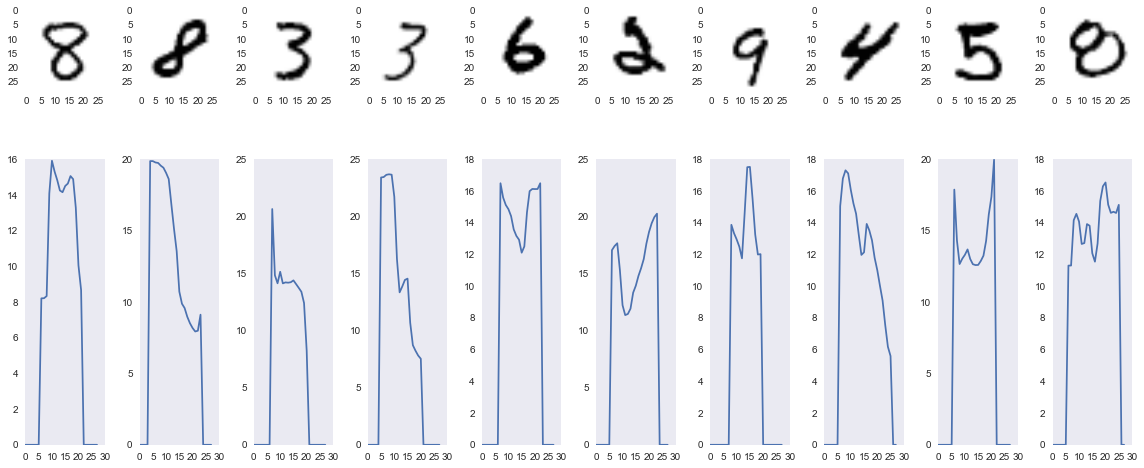
\includegraphics[width=\linewidth]{mnist_centroids.png}
        \caption{MNIST samples and centroids}
        \label{fig:mnist_centroids}
    \end{subfigure}
    \quad
    \begin{subfigure}[b]{0.4\textwidth}
        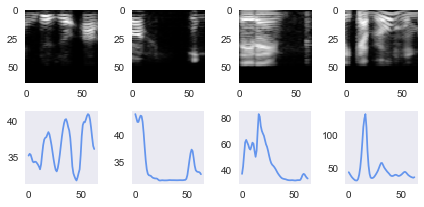
\includegraphics[width=\linewidth]{speech_spectral_centroids.png}
        \caption{Mel-Spectrograms and centroids}
        \label{fig:spectrogram_centroids}
    \end{subfigure}
    \caption{Spectral centroids on digits and Mel-Spectrograms}
    \label{fig:centroids}
\end{figure}

\subsubsection{Spectral Slope}
The spectral slope is computed by applying linear regression using a overlapping
sliding window of size 7. Figure~\ref{fig:slopes} shows these
features computed on MNIST and Mel-Spectrograms. 

\begin{figure}[!h]
    \centering
    \begin{subfigure}[b]{0.4\textwidth}
        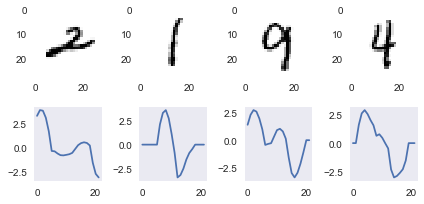
\includegraphics[width=\linewidth]{mnist_slopes.png}
        \caption{MNIST samples and slopes}
        \label{fig:mnist_slopes}
    \end{subfigure}
    \quad
    \begin{subfigure}[b]{0.4\textwidth}
        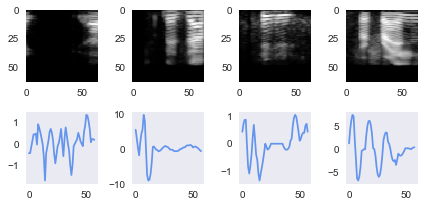
\includegraphics[width=\linewidth]{speech_spectral_slopes.png}
        \caption{Mel-Spectrograms and slopes}
        \label{fig:spectrogram_slopes}
    \end{subfigure}
    \caption{Spectral slopes on digits and Mel-Spectrograms}
    \label{fig:slopes}
\end{figure}

\subsection{Generative Models}
We investigate samples produced with the DCGAN architecture using the
Least-Squares GAN (LSGAN)~\cite{mao2016least} and the improved Wasserstein
GAN (IWGAN)~\cite{gulrajani2017improved}. We also compare adversarial MNIST
samples produced with the fast gradient sign method
(FGSM)~\cite{goodfellow2014explaining}.

%
\section{Experiments}\label{sec:experiments}
\subsection{MNIST}
We compare the distribution of features computed over the MNIST training set 
to other datasets, including
the MNIST test set, samples generated with GANs and adversarial samples computed 
using FGSM. The training data is
scaled to $[0, 1]$ and the random baseline is sampled from a Bernouli distribution with 
probability equal to the value of pixel intensities in the
MNIST training data, 0.13. Each GAN model is trained until the loss plateaus 
and the generated samples look similar to the real samples. The datasets
compared have 10 thousand samples each.

\begin{figure}[!h]
  \begin{center}
  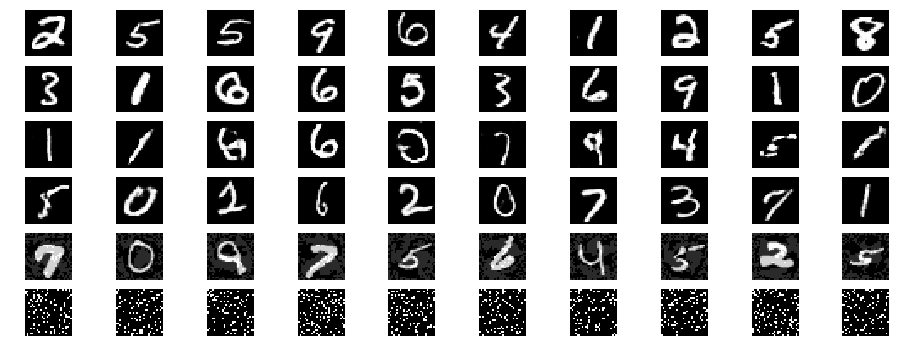
\includegraphics[width=0.8\linewidth]{mnist_samples.png}
  \caption{Samples drawn from MNIST train, test,
LSGAN, IWGAN, FSGM and bernoulli respectively.}
  \label{fig:mnist_samples}
  \end{center}
\end{figure}

Visual inspection of the generated samples in
Figure~\ref{fig:mnist_samples} show that IWGAN seems to produce better samples
than LSGAN. Quantitatively, we use the MNIST training set as a reference and compare the
distribution of pixel intensities.  Table~\ref{tbl:mnist_pixel} reveals that
although samples generated with LSGAN and IWGAN look similar to the training
set, they are considerably different from the training set given the Kolgomorov-Smirnov (KS) Two
Sample Test and the Jensen-Shannon Divergence (JSD), specially if compared to
the same statistics on the MNIST test data. 

\begin{table}[!h]
\centering
\begin{tabular}{l|ll|l|}
                   & \multicolumn{2}{c|}{\cellcolor[HTML]{C0C0C0}KS Two Sample Test} & \multicolumn{1}{c|}{\cellcolor[HTML]{C0C0C0}JSD} \\
                   & Statistic   & P-Value   &                \\
mnist\_train       & 0.0         & 1.0       & 0.0            \\
mnist\_test        & 0.003177    & 0.0       & 0.000029       \\
mnist\_lsgan       & 0.808119    & 0.0       & 0.013517       \\
mnist\_iwgan       & 0.701573    & 0.0       & 0.014662       \\
mnist\_adversarial & 0.419338    & 0.0       & 0.581769       \\
mnist\_bernoulli   & 0.130855    & 0.0       & 0.0785009      
\end{tabular}
\caption{Statistical comparisson over the distribution of pixel values for
different samples using MNIST training set as reference.}
\label{tbl:mnist_pixel}
\end{table}

These numerical phaenomena can be understood by investigating the empirical CDFs 
in Figure~\ref{fig:mnist_pixel_ecdf}. The pixel values of the samples
generated with the GAN framework are mainly bimodal and asymptotically
approach the modes of the distribution of pixel values in the real data, $0$ and $1$. Such behavior will be
present in any Generator trained using gradient descent and an asymptotically converging 
non-linearity, such as sigmoid and tanh, at the poutput of the generating function.

\begin{figure}[!h]
  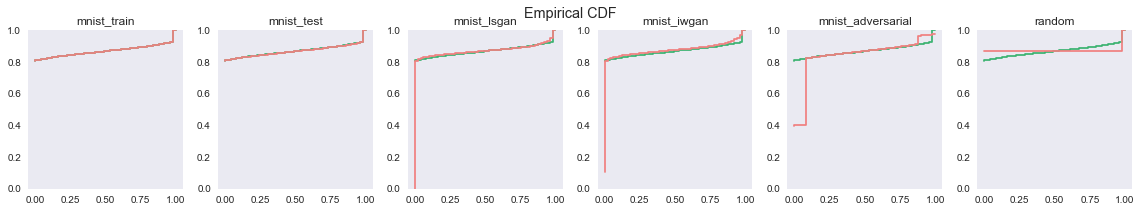
\includegraphics[width=\linewidth]{mnist_pixel_ecdf.png}
    \caption{Pixel empirical CDF of training data as reference (green) and other
    datasets(red)}
  \label{fig:mnist_pixel_ecdf}
\end{figure}

In addition, Figure~\ref{fig:mnist_pixel_distribution} shows that the GAN
generated samples smoothly approximate the modes of the distribution. This
smooth approximation is considerably different from the training and test sets.
Although these properties are not perceptually meaningful, they can be used to 
identify the source of the data, hence confirming hypotheses \ref{hyp:features}, 
\ref{hyp:visual} and \ref{hyp:difference}.

\begin{figure}[!h]
  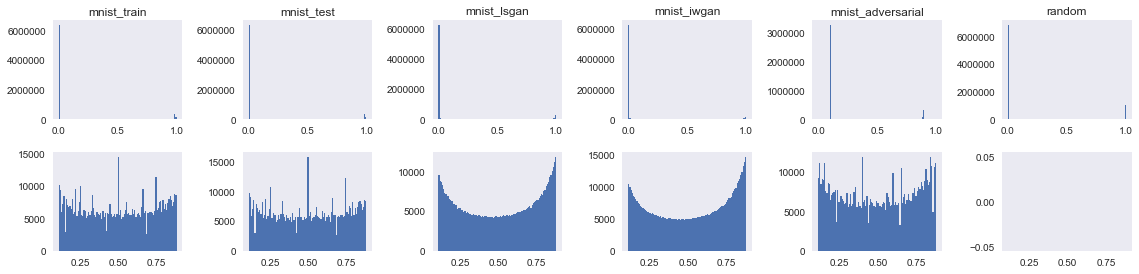
\includegraphics[width=\linewidth]{mnist_pixel_distribution.png}
  \caption{Histogram of pixel intensities for each dataset. First row shows
    histogram within the [0, 1] interval and 100 bins. Second row shows
    histograms between the [0.11, and 0.88] interval and 100 bins.}
  \label{fig:mnist_pixel_distribution}
\end{figure}

\subsection{Bach Chorales}
We investigate the properties of Bach chorales generated with the GAN framework
and verify if they satisfy musical specifications.
Bach chorales are polyphonic pieces of music, normally
written for 4 or 5 voices, that follow a set of
specifications/rules\footnote{The specifications define the characteristics of the 
musical style.}. For example, a global specification could assert that only a set of
durations are valid; a local specification could assert that only certain
transitions between states (notes) are valid depending on the current harmony.

For this experiment, we convert the dataset of Bach chorales to piano rolls. The
piano roll is a representation in which the rows represent note numbers, the columns
represent time steps and the cell values represent note intensities. We compare
the distribution of features computed over the training set, test set, GAN
generated samples and a random baseline sampled from a Bernouli distribution with 
probability equal to the normalized mean value of intensities in the
training data. After scaling, the intensities in the training and test data are
strictly bimodal and equal to $0$ or $1$. Figure~\ref{fig:chorales_samples} below
shows training, test, IWGAN and Bernoulli samples, thus confirming
hypothesis~\ref{hyp:generate}. Each dataset has roughly 1000 image patches.

\begin{figure}[!h]
  \begin{center}
  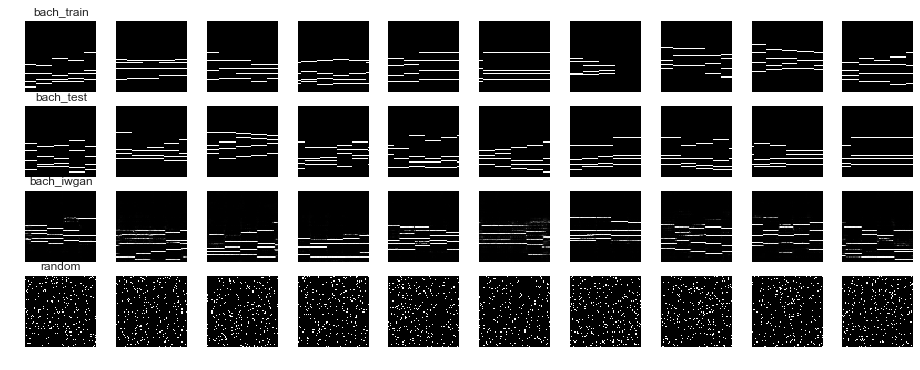
\includegraphics[width=0.8\linewidth]{chorales_samples.png}
  \caption{Samples drawn from Bach Chorales train, test,
IWGAN, and Bernoulli respectively.}
  \label{fig:chorales_samples}
  \end{center}
\end{figure}

Figure~\ref{fig:chorales_intensity_distribution} shows a behavior that is
similar to our previous MNIST experiments: the IWGAN asymtoptically approximates
the modes of the distribution of intensity values. In the 
interest of space, we refer the reader to the online appendix\footnote{Not
provided to preserve anonymity} for statistics and other relevant information. 

\begin{figure}[!h]
  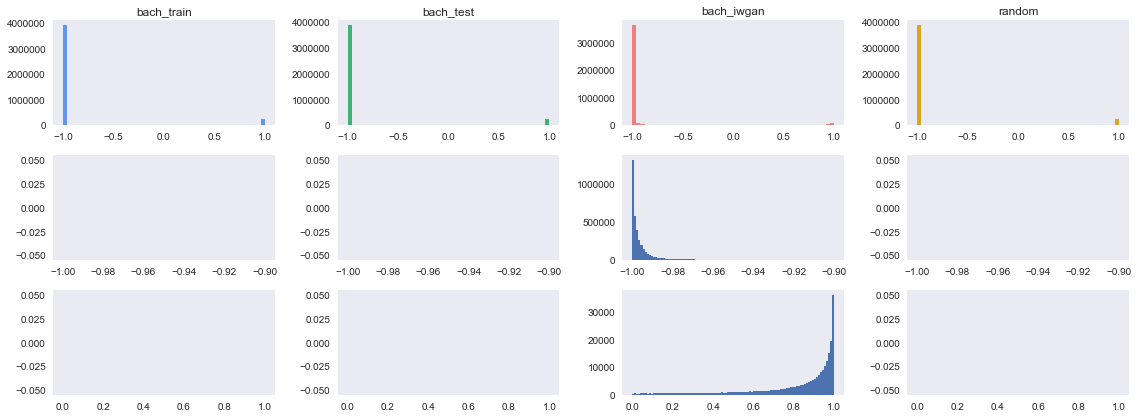
\includegraphics[width=\linewidth]{chorales_intensity_distribution.png}
  \caption{}
  \label{fig:chorales_intensity_distribution}
\end{figure}

Following, we investigate if the generated samples violate the specifications of
Bach chorales. For doing so, we first convert all datasets to boolean by 
thresholding at 0.5 such that values above the threshold are set to 1 or 0
otherwise. We use
these piano rolls to compute boolean Chroma~\cite{peeters2004large} feature and
to compute an empirica Chroma transition matrix, where the positive
entries represent existing and valid transitions. The transition matrix built on 
the training data is taken as the reference specification, i.e. anything that is 
not included is a violation of the specification. Table~\ref{tbl:chroma_violations}
shows the number of violations given each dataset. Although
Figure~\ref{fig:chorales_samples} shows generated samples that look similar to
the real data, the IWGAN samples have over 5000
violations, 10 times more than the test set! We use these facts to confirm
hypotheses \ref{hyp:features}, \ref{hyp:visual} and \ref{hyp:difference}.

\begin{table}[!h]
\centering
\begin{tabular}{lllll}
& \cellcolor[HTML]{C0C0C0}bach\_train & \cellcolor[HTML]{C0C0C0}bach\_test & \cellcolor[HTML]{C0C0C0}bach\_iwgan & \cellcolor[HTML]{C0C0C0}bach\_bernoulli \\ \cline{2-5} 
\multicolumn{1}{l|}{\cellcolor[HTML]{C0C0C0}Number of Violations} & 0                                   & 429                                & 5029                                & 58284                                  
\end{tabular}
\caption{Number of specification violations with training data as
    reference.}
\label{tbl:chroma_violations}
\end{table}

In addition to experiments with Chroma features, we computed the distribution of
note durations on the boolean piano roll described above.
Figure~\ref{fig:chorales_duration_distribution} shows the distribution of
note durations within each dataset. The train and test data are approximatelly
bimodal and, again, the improved WGAN smoothly approximates the
dominating modes of the distribution. Table~\ref{tbl:duration} provides a numerical 
comparisson between datasets.


\begin{figure}[!h]
    \begin{subfigure}[b]{0.65\textwidth}
        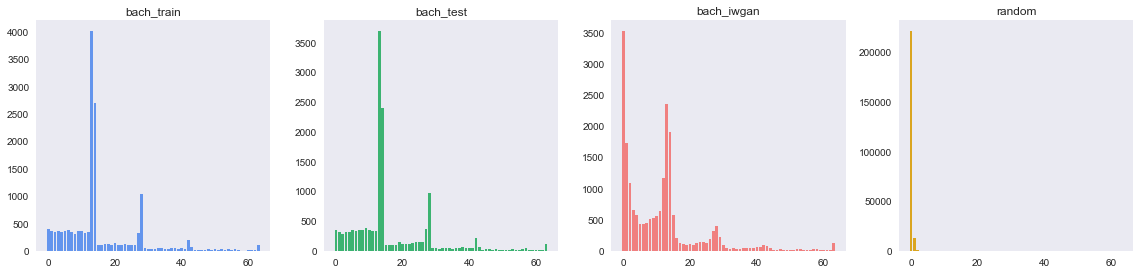
\includegraphics[width=\linewidth]{chorales_duration_distribution.png}
        \caption{Histogram of note durations}
        \label{fig:chorales_duration_distribution}
    \end{subfigure}
    \quad
    \begin{subfigure}[b]{0.3\textwidth}
    %\begin{table}[!h]
        \resizebox{1.0\textwidth}{!}{%
        \begin{tabular}{l|ll|l|}
                           & \multicolumn{2}{c|}{\cellcolor[HTML]{C0C0C0}KS Two Sample Test} & \multicolumn{1}{c|}{\cellcolor[HTML]{C0C0C0}JSD} \\
                           & Statistic   & P-Value  &         \\
        train       & 0.0          & 1.0      & 0.0     \\
        test        & 0.09375      & 0.929    & 0.002   \\
        iwgan       & 0.21875      & 0.080    & 0.084   \\
        bernoulli   & 0.93750      & 0.0      & 0.604   
        \end{tabular}
        }
        \caption{Test statistics}
        \label{tbl:duration}
    %\end{table}
    \end{subfigure}
\end{figure}

\subsection{Speech}
Within the speech domain, we investigate dynamic compressed Mel-Spectrogram 
samples produced with GANs trained on a subset of the NIST 2004 dataset, with
100 speakers. We divide the NIST 2004 dataset into training and test set,
generate samples with the GAN framework and use a random baseline sampled from 
a Exponential distribution with parameters chosen using heuristics.
The generated samples can be seen in
Figure~\ref{fig:speech_samples}, thus confirming hypothesis~\ref{hyp:generate}.
We obtain the Mel-Spectrogram by projecting a
spectrogram onto a mel scale, which we do with the python library
librosa~\cite{mcfee2015librosa}. More specifically,  we project the spectrogram 
onto 64 mel bands,
with window size equal to 1024 samples and hop size equal to 160 samples, i.e.
frames of 100ms long. Dynamic range compression is computed as described 
in~\cite{lukic2016speaker}, with $log(1 + C*M)$, where $C$ is the compression 
constant scalar set to $1000$ and $M$ is the matrix representing the Mel-Spectrogram.
Each dataset has approximately 1000 image pataches and the GAN models are trained 
using DCGAN with the improved Wasserstein GAN algorithm.

\begin{figure}[!h]
  \begin{center}
  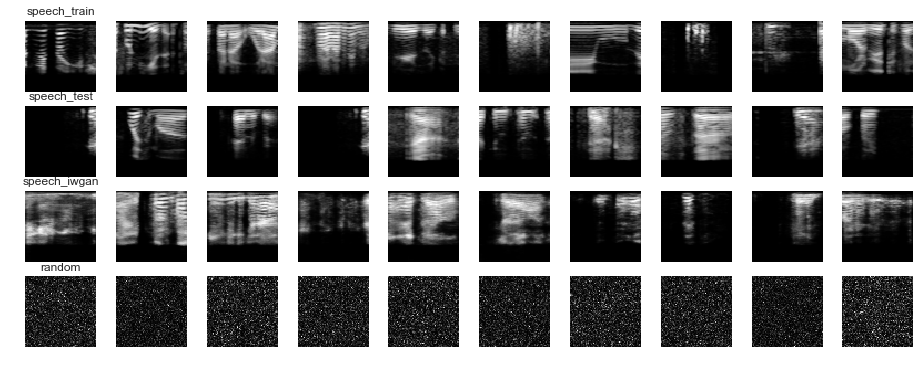
\includegraphics[width=0.8\linewidth]{speech_samples.png}
  \caption{Samples drawn from Mel-Spectrogram Speech train, test,
IWGAN, and exponential respectively.}
  \label{fig:speech_samples}
  \end{center}
\end{figure}

In Figure~\ref{fig:speech_intensity_ecdf} we show the empirical CDFs of intensity
values. Unlike our previous experiments where intensity (Bach Chorales)
or pixel value (MNIST) was linear, in this experiment intensities are compressed using the
log function. This considerably reduces the distance between the empirical CDFs
of the training data and GAN samples,
specially around the saturating points of the tanh non-linearity, $-1$ and $1$ in this
case. In Table~\ref{tbl:speech_intensity} we show numerical analysis of the
differences and confirm hypotheses \ref{hyp:features} and \ref{hyp:visual}.
\begin{figure}[!h]
    \begin{subfigure}[b]{0.65\textwidth}
        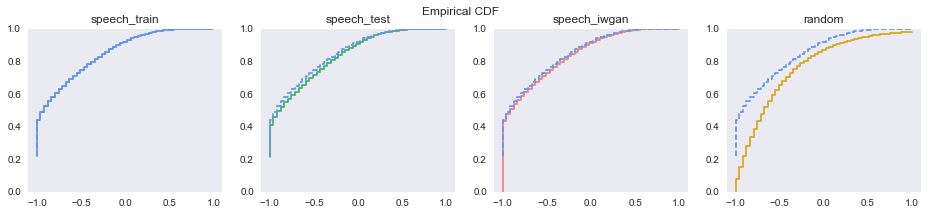
\includegraphics[width=1.0\linewidth]{speech_intensity_ecdf.png}
        \caption{Intensity empirical CDF of training data in blue
        and other datasets.}
        \label{fig:speech_intensity_ecdf}
    \end{subfigure}
    \quad
    \begin{subfigure}[b]{0.3\textwidth}
    %\begin{table}[!h]
        \resizebox{1.0\textwidth}{!}{%
        \begin{tabular}{l|ll|l|}
                           & \multicolumn{2}{c|}{\cellcolor[HTML]{C0C0C0}KS Two Sample Test} & \multicolumn{1}{c|}{\cellcolor[HTML]{C0C0C0}JSD} \\
                    & Statistic    & P-Value  &         \\
        train       & 0.0          & 1.0      & 0.0     \\
        test        & 0.03685      & 0.0      & 0.00080   \\
        iwgan       & 0.22149      & 0.0      & 0.00056   \\
        bernoulli   & 0.36205      & 0.0      & 0.11423   
        \end{tabular}
        }
        \caption{Test statistics}
        \label{tbl:speech_intensity}
    %\end{table}
    \end{subfigure}
    \caption{Empirical CDF and statistical tests of speech intensity}
    \label{fig:speech_intensity}
\end{figure}

Figure~\ref{fig:speech_moments} shows the distribution of statistical moments computed on
spectral centroids and slope. The distributions from different sources
considerably overlap, indicating that the generator has efficiently approximated
the real distribution of these features.

\begin{figure}[!h]
    \centering
    \begin{subfigure}[b]{0.45\textwidth}
        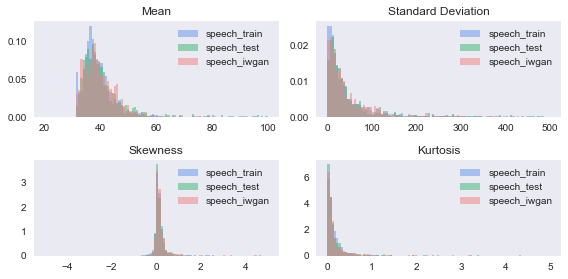
\includegraphics[width=\linewidth]{speech_spectral_centroid_moments.png}
        \caption{Spectral Centroid Moments}
        \label{fig:speech_spectral_centroid_moments}
    \end{subfigure}
    \quad
    \begin{subfigure}[b]{0.45\textwidth}
        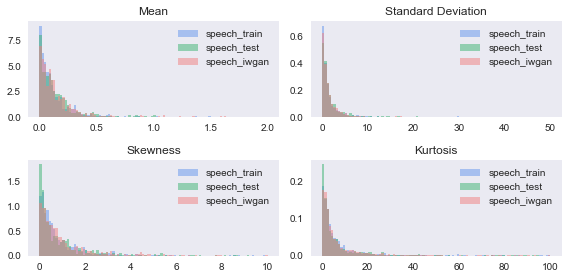
\includegraphics[width=\linewidth]{speech_spectral_slope_moments.png}
        \caption{Spectral Slope Moments}
        \label{fig:speech_spectral_slope_moments}
    \end{subfigure}
    \caption{Moments of spectral centroid (left) and slope(right)}
    \label{fig:speech_moments}
\end{figure}

Figure~\ref{fig:speech_spectral_stats} shows statistics used to compare the
reference (training data) and other datasets. The difference between
KS-Statistics and JSD of the test data and generated samples are negligible.
Interestingly, the p-values of the spectral slope of the improved WGAN are considerably
higher than the test data. For these reasons and although 
Table~\ref{tbl:speech_intensity} shows a significant difference between the 
KS-Statistic of test data and generated data with respect to the training
data, we refrain from confirming hypothesis \ref{hyp:difference}. An adversary
can easily manipulate the generated data to considerably decrease 
this difference and still keep the high similarity in features harder to
simulate such as moments of spectral centroid or slope. 

\begin{figure}[!h]
    \centering
    \begin{subfigure}[b]{.45\textwidth}
        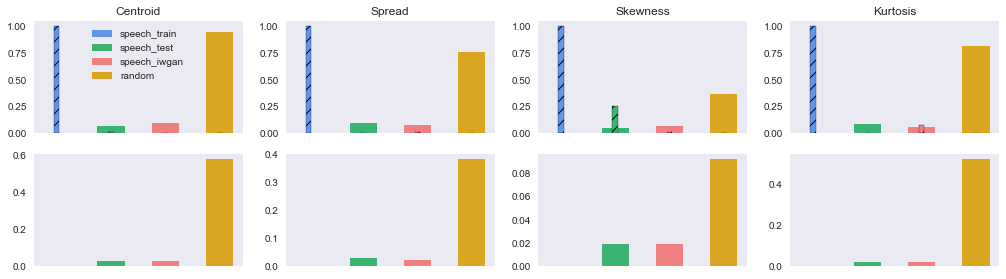
\includegraphics[width=\linewidth]{speech_spectral_centroid_stats.png}
        \caption{Spectral Centroid Statistics}
        \label{fig:speech_spectral_centroid_stats}
    \end{subfigure}
    \quad
    \begin{subfigure}[b]{.45\textwidth}
        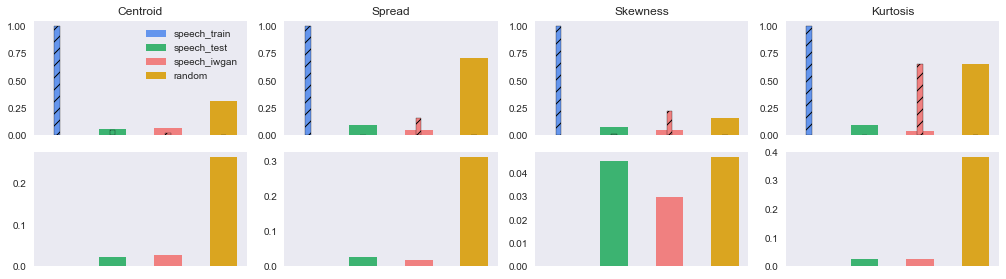
\includegraphics[width=\linewidth]{speech_spectral_slope_stats.png}
        \caption{Spectral Slope Statistics}
        \label{fig:speech_spectral_slope_stats}
    \end{subfigure}
    \caption{Statistics of spectral centroid (left) and slope(right)}
    \label{fig:speech_spectral_stats}
\end{figure}

%
\section{Conclusions}\label{sec:conclusions}
In this paper we investigated numerical properties of samples produced 
with adversarial methods, specially Generative Adversarial Networks. We showed that GAN samples have universal signatures that are dependent on the choice of non-linearity on the last layer of the generator. In addition, we showed that adversarial examples produced with the FSGM have properties that can be used to identify an adversarial attack. Following, we showed that GAN samples smoothly approximate the dominating modes of the distribution and that this information can be used to identify the source of the data. Finally, we showed that samples generated with GANs do not provide guarantees on satisfaction of simple specifications. With this we hope to call attention to our community to the necessity of developing a theory of verifiable artificial intelligence.
%

\subsubsection*{Acknowledgments}
\input{acknowledgments}

\bibliographystyle{plain}
\bibliography{references}

\end{document}
